\chapter{矩阵运算进阶}

\section{分块矩阵}
\subsection{运算性质}
\begin{definition}
	一般的,对于$m \times n$矩阵$A$,如果在行的方向分成$s$块,在列的方向分成$t$
	块,就得到$A$的一个$s \times t$分块矩阵,记作$A=(A_{kl})_{s \times t}$,其中
	$A_{kl}(k=1,\cdots,s;l=1,\cdots,t)$称为$A$的子块.
\end{definition}
实际上上述表示方法就是将一般矩阵表示$A=(a_{ij})_{m \times n}$中的$a_{ij}$替换为了小块矩阵,
字母含义并无变化,内层代表索引,外层代表总行列数(只是分块矩阵是块索引和块数).
我们接下来考察分块矩阵的运算性质.

1. 分块矩阵的加法:设分块矩阵$A=(A_{kl})_{s \times t}$,$B=(B_{kl})_{s \times t}$,如果$A$与$B$
对应的子块$A_{kl}$和$B_{kl}$都是同型矩阵,则$$A+B=(A_{kl}+B_{kl})_{s \times t}.$$
由此我们看到分块矩阵加法要求小块形状和行列分块数都一致,实际上回顾一般矩阵加法要求矩阵完全同型即可理解这一要求.

2. 分块矩阵的数乘:设分块矩阵$A=(A_{kl})_{s \times t}$,$\lambda$是一个数,则
$$\lambda A=(\lambda A_{kl})_{s \times t}.$$
实际上数乘最好理解,因为如此计算的效果相当于一般矩阵数乘的效果,即给每个元素
都乘以一个常数$\lambda$.

3. 分块矩阵的乘法:设$A=(a_{ij})_{m \times n}$,$B=(b_{ij})_{n \times p}$,如果
把$A$,$B$分别分块为$r \times s$和$s \times t$分块矩阵,且$A$的列分块法与$B$的行分块法相同
(注意这些条件始终保证可乘性成立),则
$$AB=\begin{pmatrix}
	A_{11} & A_{12} & \cdots & A_{1s} \\
	A_{21} & A_{22} & \cdots & A_{2s} \\
	\cdots &  &  & \cdots \\
	A_{r1} & A_{r2} & \cdots & A_{rs}
\end{pmatrix}\begin{pmatrix}
	B_{11} & B_{12} & \cdots & B_{1t} \\
	B_{21} & B_{22} & \cdots & B_{2t} \\
	\cdots &  &  & \cdots \\
	B_{s1} & B_{s2} & \cdots & B_{st}
\end{pmatrix}=C=(C_{kl})_{r \times t}.$$
其中$C$是$r \times t$分块矩阵,且$C_{kl}$与一般矩阵计算类似,即为$A$第$k$行块$B$的$l$列块对应元素相乘后相加,即
$$C_{kl}=A_{k1}B_{1l}+A_{k2}B_{2l}+\cdots+A_{ks}B_{sl},\ k=1,\cdots,r;l=1,\cdots,t.$$

4. 分块矩阵的转置:大、小矩阵都要转置,这是分块矩阵与普通矩阵的一大性质差异;即$s \times t$分块矩阵$A=(A_{kl})_{s \times t}$
转置后$A^\mathrm{T}=(B_{lk})_{t \times s}$为$t \times s$分块矩阵,且$B_{lk}=A_{kl}^\mathrm{T}$.
例如$\begin{pmatrix}
	A_{11} & A_{12} \\ A_{21} & A_{22}
\end{pmatrix}^\mathrm{T}=\begin{pmatrix}
	A_{11}^\mathrm{T} & A_{21}^\mathrm{T} \\ A_{12}^\mathrm{T} & A_{22}^\mathrm{T}
\end{pmatrix}$.

补充以下注意事项:

1. 常见的行列分块方法:将矩阵按行/列分块,注意$A(\beta_1,\cdots,\beta_n)=(A\beta_1,\cdots,A\beta_n)$成立,
但当$A$在右侧时并不可乘,按行分块也有对称的结论;

2. 注意分块矩阵求逆,可以直接使用设未知数的方式完成,也可以利用下面即将介绍的分块矩阵初等变换进行解决;

3. 分析分块矩阵与普通矩阵的运算性质的异同:分块矩阵转置需要注意大小都要转置,注意分块矩阵每一块仍为矩阵,所以当普通矩阵元素的求倒数
对应于小块的求逆,加法乘法一定要块对应等,但实际上其他很多性质都是将单个元素推广为一块.
\begin{example}
	设$$A=\begin{pmatrix}
		1 & 2 & 0 & 0 & 0 \\
		2 & 5 & 0 & 0 & 0 \\
		0 & 0 & -2 & 1 & 0 \\
		0 & 0 & 0 & -2 & 1 \\
		0 & 0 & 0 & 0 & -2
	\end{pmatrix},\ B=\begin{pmatrix}
		1 & 0 & 1 & 0 \\
		-1 & 2 & 3 & 0 \\
		1 & 2 & 0 & 4 \\
		0 & 1 & 2 & 4 \\
		0 & 0 & 1 & 4
	\end{pmatrix}.$$
	利用分块矩阵的方法,求$A^2,\ AB,\ A^\mathrm{T},\ A^{-1}$.
\end{example}
\subsection{分块矩阵初等变换(打洞法)*}
分块矩阵的初等变换实际上可以视为一般矩阵初等变换的推广,实际上也有三种相应的推广形式,
即交换两行、对某一行乘以一个可逆矩阵以及对某一行左乘矩阵后加到另一行.它们的计算性质
以及可逆性质的证明比较繁琐,我们这里略去,直接应用即可.实际使用的时候,很多时候都是
使用一种将分块矩阵中的小块视为常数来处理.

分块矩阵初等行变换的一个重要的应用就是“打洞法”,常用于分块矩阵求逆的运算,在之后行列式的一些技巧性处理中也很常见.
例如:
\begin{enumerate}
	\item 当$A$可逆时,我们可以通过初等行变换消去$C$:
	$$\begin{pmatrix}
		E & O \\ -CA^{-1} & E
	\end{pmatrix}\begin{pmatrix}
		A & B \\ C & D
	\end{pmatrix}=\begin{pmatrix}
		A & B \\ O & D-CA^{-1}B
	\end{pmatrix}$$
	可以继续做列变换消去$B$:
	$$\begin{pmatrix}
		A & B \\ O & D-CA^{-1}B
	\end{pmatrix}\begin{pmatrix}
		E & -A^{-1}B \\ O & E
	\end{pmatrix}=\begin{pmatrix}
		A & O \\ O & D-CA^{-1}B
	\end{pmatrix}$$
	\item 特别地,对于对称矩阵$\begin{pmatrix}A & B \\ B^\mathrm{T} & D\end{pmatrix}$,其中$A$和$D$也是对称方阵,
	则$A$可逆时,可以通过合同变换消除$B$和$B^\mathrm{T}$,即
	$$\begin{pmatrix}
		E & -A^{-1}B \\ O & E
	\end{pmatrix}^\mathrm{T}\begin{pmatrix}
		A & B \\ B^\mathrm{T} & D
	\end{pmatrix}\begin{pmatrix}
		E & -A^{-1}B \\ O & E
	\end{pmatrix}=\begin{pmatrix}
		A & O \\ O & D-B^\mathrm{T}A^{-1}B
	\end{pmatrix}$$
\end{enumerate}
接下来求取逆矩阵就很容易了,因为分块对角矩阵求逆矩阵就是对每个小对角块求逆,十分简单,所以解决此类问题
首先要利用分块矩阵初等变换进行对角化(一定注意区分行列变换的左右乘),然后如果$PAQ=\Lambda$,
其中$P$和$Q$为分块初等矩阵,$\Lambda$为分块对角矩阵,利用分块对角矩阵的逆容易计算的
特点计算$Q^{-1}A^{-1}P^{-1}=\Lambda^{-1}$,即可得到$A^{-1}=Q\Lambda^{-1}P$.
\begin{example}
	当$D$可逆时,仿照上面的步骤对角化分块矩阵$\begin{pmatrix}A & B \\ C & D\end{pmatrix}$并求逆矩阵.
\end{example}

\subsection{分块矩阵与数学归纳法}
分块矩阵经常运用在数学归纳法中,我们在之后的课程中也会经常用到这样的思想,
这一思想基于以下内容:

对于$\begin{pmatrix}
	A_1 & \alpha \\ \beta & a_{nn}
\end{pmatrix}$,假设$A_1$可逆,我们有
$$\begin{pmatrix}
	E_{n-1} & 0 \\ -\beta A_1^{-1} & 1
\end{pmatrix}\begin{pmatrix}
	A_1 & \alpha \\ \beta & a_{nn}
\end{pmatrix}=\begin{pmatrix}
	A_1 & \alpha \\ 0 & a_{nn}-\beta A_1^{-1}\alpha
\end{pmatrix}$$

\begin{example}
	若$n$阶矩阵$A$的各阶左上角子块矩阵都可逆,则存在主对角元全为$1$的下三角矩阵$L$和上三角矩阵$U$,使得$A=LU$($L$-$U$分解).
\end{example}

\section{特殊矩阵}
本节将会介绍一些常见的特殊矩阵以及它们常用的基本性质,还有一些将在特征值专题中讲解.
\subsection{对角矩阵}
我们一般记主对角矩阵为$\textup{diag}(d_1,d_2,\dots,d_n)$,准对角矩阵为$\textup{diag}(A_1,A_2,\dots,A_n)$.
下面是对角矩阵的一个基本定理,它很简单,但是很重要:
\begin{theorem}
	设$A$是一个$s \times n$矩阵,把$A$写成列向量与行向量的形式,分别为
	\begin{figure}[h]
		\centering
		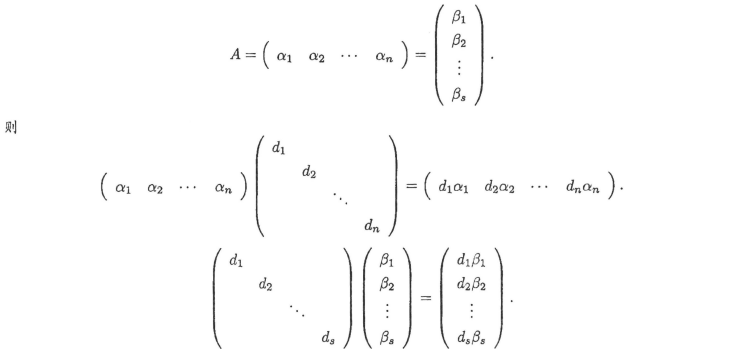
\includegraphics[scale=0.6]{./figs/9/9-1.png}
	\end{figure}
	
	即$A$右乘对角矩阵$\textup{diag}(d_1,d_2,\dots,d_n)$相当于给$A$的第$i$列元素都乘以$d_i$,
	$A$左乘对角矩阵$\textup{diag}(d_1,d_2,\dots,d_n)$相当于给$A$的第$i$行元素都乘以$d_i$.
\end{theorem}
\begin{theorem}
	(请自行完成以下内容的补充)

	对角矩阵以及准对角矩阵的三则运算、可逆性以及逆运算、乘方运算等规则.
\end{theorem}

\subsection{上(下)三角矩阵}
\begin{theorem}
	已知$A$,$B$都是上三角矩阵,且设$A$的主对角元素分别为$a_{11},\dots,a_{nn}$,B的主对角元素分别为
	$b_{11},\dots,b_{nn}$,则
	
	\textup{(1)}$A^{\mathrm{T}}$,$B^\mathrm{T}$都是下三角矩阵;
	
	\textup{(2)}$AB$仍然是上三角矩阵,且$AB$的主对角元素为$a_{11}b_{11},\dots,a_{nn}b_{nn}$;
	
	\textup{(3)}$A$可逆的充要条件是其主对角元均不为$0$,且$A$可逆时,$A^{-1}$也是上三角矩阵,并且$A^{-1}$的主对角元素分别为$a_{11}^{-1},\dots,a_{nn}^{-1}$.
\end{theorem}

\begin{example}
	已知$A_1,\dots,A_n$是$n$个对角元都为$0$的上三角矩阵,证明:$A_1A_2\dots A_n=O$.
\end{example}

\subsection{基本矩阵}
只有一个元素为1,其余元素全为0的矩阵称为基本矩阵,第$i$行第$j$列元素为1的基本矩阵记为$E_{ij}$,
他们具有如下性质(可以回忆左右乘对应行列变换):
\begin{theorem}

	\textup{(1)}$AE_{ij}$的结果就是把$A$的第$i$列移到第$j$列的位置,其余元素都为$0$的矩阵;
	
	\textup{(2)}$E_{ij}B$的结果就是把$B$的第$j$行移到第$i$行的位置,其余元素都为$0$的矩阵;
	
	\textup{(3)}$E_{ik}E_{kj}=E_{ij}$,当$k \neq l$时,有$E_{ik}E_{lj}=O$.
\end{theorem}

\subsection{其他矩阵}
其他矩阵如正交矩阵、置换矩阵、幂等矩阵、幂零矩阵等,有的会在稍后介绍部分性质,有的
则会在课程进行中或者后续课程中再见到它们.

\section{矩阵的逆进阶求法}
\subsection{给定多项式求逆矩阵}
此类题目相信大家已经有所见识,实际上就是通过一些初中所学的因式分解等基本变换得到需要求逆的矩阵与另一个矩阵相乘
可以得到单位矩阵(的一个倍数).
\begin{example}
	设$A$为非零矩阵,且$A^3=O$,证明:$E+A$和$E-A$都可逆.
\end{example}

\begin{example}
	若$X$,$Y$是两个列向量,且$X^\mathrm{T}Y=2$,证明:

	\textup{(1)}$(XY^\mathrm{T})^k=2^{k-1}(XY^{\mathrm{T}})$;

	\textup{(2)}如果$A=E+XY^\mathrm{T}$,则$A$可逆,并求其逆矩阵.

\end{example}

\subsection{利用分块矩阵初等变换*}
我们在前面已经讲解过了打洞法的基础题型,这里再给出一些例子:
\begin{example}
	设$A$、$B$为$n$阶矩阵,证明:若$E\pm AB$可逆,则$E\pm BA$可逆.
\end{example}
\begin{example}
	设$A$为$n$阶矩阵,$B$、$C$分别为$n \times m$、$m \times n$阶矩阵,
	证明:$E_m+CA^{-1}B$可逆$\iff A+BC$可逆.
\end{example}

\subsection{求逆的分式思想*}
虽然矩阵没有除法运算,但是我们如果将$(E-A)^{-1}$写成$\frac{E}{E-A}$,再类比泰勒展开
$$\frac{1}{1-x}=1+\sum_{n=1}^\infty x^n(x\in (-1,1))$$我们可以得到(不严谨!只能用来解题的时候当作初步的思路!)
$$(E-A)^{-1}=\frac{E}{E-A}=E+A+A^2+\dots$$

\begin{example}
	已知方阵$A$满足$A^k=O$,其中$k$是一个正整数,求$E-A$的逆.
\end{example}

\begin{example}
	设$A$,$B$分别是$n \times m$和$m \times n$的矩阵,且$E_n \pm AB$可逆,则$E_m \pm BA$可逆.
\end{example}
不难发现这一例是前述4.3.1节中最后一个例题的推广.

\subsection{提逆思想*}
这一思想的来源是矩阵逆没有加减相关的运算法则,因此我们需要提逆产生一些乘积项来解决问题.
\begin{example}
	设$A$是$n$阶方阵,且$E-A$,$E+A$和$A$都可逆,证明:$(E-A^{-1})^{-1}+(E-A)^{-1}=E$.
\end{example}

\section{矩阵的迹*}
\subsection{基本概念与性质}
\begin{definition}
	一个方阵$A$的所有主对角元素之和称为$A$的迹,记为$\textup{tr}(A)$.
\end{definition}
迹的常见性质如下:
\begin{theorem}
	已知$A$,$B$是两个$n$阶矩阵,$k$是一个常数,则

	\textup{(1)}\textup{tr}$(kA)$=$k$\textup{tr}$(A)$;

	\textup{(2)}\textup{tr}$(A+B)$=\textup{tr}$(A)+$\textup{tr}$(B)$;
	
	\textup{(3)}\textup{tr}$(AB)$=\textup{tr}$(BA)$;
	
	\textup{(4)}如果$A$是实矩阵,则$A=O \iff$\textup{tr}$(A^{\mathrm{T}}A)=0$.
\end{theorem}

我们先来看一个基本的例子练习一下:
\begin{example}
	证明:不存在方阵$A$、$B$使得$AB-BA=E$.
\end{example}

接下来我们介绍一个性质,这一性质的证明需要利用矩阵的秩中讲到的一些技巧:
\begin{theorem}
	已知 $n$ 阶矩阵 $A$ 的秩为 $1$ ,证明:$A^k=\textup{tr}(A)^{k-1}A$.
\end{theorem}
这一定理的证明需要用到矩阵的分解,在2020年吴志祥老师班期中考试有出现,可以参考
辅学网站上的解答.

当然我们还会在特征值一章再次见到矩阵的迹,相关内容在最后一个专题会展开讲述.

\subsection{幂零矩阵}
幂零矩阵是一种特殊的矩阵,幂零矩阵$A$存在一个正整数$k$使得$A^k=O$,
它具有如下性质(部分需要用到特征值,所以最后一个专题还会提及):
\begin{theorem}
	若$n$阶矩阵$A$为幂零矩阵,则

	\textup{(1)}$A^n=O$;

	\textup{(2)}$A\pm E$均为可逆矩阵;

	\textup{(3)}幂零矩阵对应的线性变换一定存在一个矩阵表示使得矩阵为上三角矩阵且对角线元素全为\textup{0};
	
	\textup{(4)}$A$为幂零矩阵$\iff \forall k \in N^+$,\textup{tr}$(A^k)$=\textup{0}.
\end{theorem}

\begin{example}
	若$A$、$B$为两个$n$阶矩阵且满足$AB-BA=A$,证明:

	\textup{(1)}$A$不可逆;

	\textup{(2)}$A$是幂零矩阵.
\end{example}

\section{矩阵的幂}
\begin{enumerate}
	\item 找规律
	
	在矩阵的转置中我们已经见识了一种找规律的方式,下面是一种类似的题型:
	\begin{example}
		计算$(PAQ)^k$,其中
		$$P=\begin{pmatrix}2 & 3 \\ 1 & 2\end{pmatrix}, A=\begin{pmatrix}2 & 0 \\ 0 & -1\end{pmatrix}, Q=\begin{pmatrix}2 & -3 \\ -1 & 2\end{pmatrix}$$
	\end{example}
	
	\begin{example}
		设$A=\begin{pmatrix}0 & -1 & 0 \\ 1 & 0 & 0 \\ 0 & 0 & -1 \end{pmatrix}$,
		$P^{-1}AP=B$,求$B^{2004}-2A^2$.
	\end{example}

	还有一种找规律基于幂等矩阵,显然幂等矩阵的任意次方都与其平方相等是很好的性质,另一种找规律基于对合矩阵,即平方等于单位矩阵的矩阵,我们这里
	主要与大家分享关于幂零矩阵的方法,例子如下:
	\begin{example}
		求$A=\begin{pmatrix}a & 1 & 0 & 0 \\ 0 & a & 1 & 0 \\ 0 & 0 & a & 0 \\ 0 & 0 & 0 & a \end{pmatrix}^n$.
	\end{example}
	在上例中,我们采用将矩阵分为$A=tE+B$的方法,会发现矩阵$B$为上三角矩阵且对角线上全为0,是典型的幂零矩阵,利用这一性质可以快速解题.
	\item 数学归纳法
	\begin{example}
		求$A=\begin{pmatrix}\cos\alpha & \sin\alpha \\ -\sin\alpha & \cos\alpha\end{pmatrix}^n$.
	\end{example}
	这一问题对应我们常见的旋转变换.
	\begin{example}
		证明$\begin{pmatrix}
			a & c \\ 0 & b
		\end{pmatrix}^n=\begin{pmatrix}
			a^n & (a^{n-1}+a^{n-2}b+\dots+b^{n-1})c \\ 0 & b^n
		\end{pmatrix}$.
	\end{example}
	\item 利用秩为1的矩阵
	
	在我们有关秩的讨论中已经提到了如果$A$是秩为1的矩阵,那么$A^n=(\textup{tr}(A))^{n-1}A$,我们可以利用这一性质解决问题.
	\begin{example}
		已知$M$是秩为$1$的矩阵,记\textup{tr}$(M)=b$,讨论$(aE+M)^n$的计算结果.
	\end{example}

	\begin{example}
		已知$A$是数域$P$上的一个$2$阶方阵,且存在正整数$l$使得$A^l=O$,证明:$A^2=O$.
	\end{example}
	事实上,我们在幂零矩阵的讨论中已经提及了上例的一般情况.

	\begin{example}
		已知数列$\{a_n\}$,$\{b_n\}$满足$a_0=-1$,$b_0=3$,且
		$$\begin{cases}
			a_n=3a_{n-1}+b_{n-1}+2^{n-1} \\ b_n=2a_{n-1}+4b_{n-1}+2^n
		\end{cases}$$
		求$\{a_n\}$,$\{b_n\}$的通项公式.
	\end{example}
	\item 利用初等矩阵的性质
	\begin{example}
		设$A$为三阶矩阵,$P$为三阶可逆矩阵,$P^{-1}AP=B$,其中$P=\begin{pmatrix}
			0 & 2 & -1 \\ 1 & 1 & 2 \\ -1 & -1 & -1
		\end{pmatrix}$,$B=\begin{pmatrix}
			0 & 0 & -1 \\ 0 & -1 & 0 \\ -1 & 0 & 0
		\end{pmatrix}$,求$A^{2022}$.
	\end{example}

	\item 利用对角化
	
	若一个矩阵$A$可对角化,即存在可逆矩阵$P$使得$A=P^{-1}\Lambda P$(其中$\Lambda$为对角矩阵),
	在这种形式下$A$的幂是很好求的.
	\begin{example}
		已知$A=\begin{pmatrix}
			0 & \cfrac{1}{2} & \cfrac{1}{2} \\ 1 & -\cfrac{1}{2} & \cfrac{1}{2} \\ 1 & -\cfrac{1}{2} & \cfrac{1}{2}
		\end{pmatrix}$,求$A^n$.
	\end{example}

\end{enumerate}

\vspace{2ex} 
\centerline{\heiti \Large 内容总结}

\vspace{2ex} 

\centerline{\heiti \Large 习题}
\vspace{2ex} 
{\kaishu }
\begin{flushright}
    \kaishu

\end{flushright}
\centerline{\heiti A组}
\begin{enumerate}
	\item 
\end{enumerate}
\centerline{\heiti B组}
\begin{enumerate}
	\item 
\end{enumerate}
\centerline{\heiti C组}
\begin{enumerate}
	\item 
\end{enumerate}